\documentclass[12pt, a4paper]{report}
\usepackage[top=1cm, left=1cm, right=1cm]{geometry}

\usepackage[utf8]{inputenc}
\usepackage[russian]{babel}

\usepackage{array}
\newcolumntype{M}[1]{>{\centering\arraybackslash}m{#1}}

\usepackage{hyperref}
\hypersetup{
	colorlinks,
	citecolor=black,
	filecolor=black,
	linkcolor=black,
	urlcolor=black
}

\usepackage{sectsty}
\allsectionsfont{\centering}

\usepackage{indentfirst}
\setlength\parindent{24pt}

\usepackage{algorithm}
\usepackage[noend]{algpseudocode}

\usepackage{listings}
\usepackage{xcolor}
\definecolor{codegreen}{rgb}{0,0.6,0}
\definecolor{codegray}{rgb}{0.5,0.5,0.5}
\definecolor{codepurple}{rgb}{0.58,0,0.82}
\definecolor{backcolour}{rgb}{0.95,0.95,0.92}
\lstdefinestyle{mystyle}{
    backgroundcolor=\color{backcolour},
    commentstyle=\color{codegreen},
    keywordstyle=\color{magenta},
    numberstyle=\normalsize\color{codegray},
    stringstyle=\color{codepurple},
    basicstyle=\ttfamily\footnotesize,
    breakatwhitespace=false,
    breaklines=true,
    captionpos=b,
    keepspaces=true,
    numbers=left,
    numbersep=5pt,
    showspaces=false,
    showstringspaces=false,
    showtabs=false,
    tabsize=2
}

\usepackage{graphicx}
\graphicspath{ {plots/pictures/}{assets/pictures} }

\begin{document}
	\begin{titlepage}
		\begin{center}
			\large \textbf{Министерство науки и высшего образования Российской Федерации} \\
			\large \textbf{Федеральное государственное бюджетное образовательное учреждение высшего образования} \\
			\large \textbf{«Российский химико-технологический университет имени Д.И. Менделеева»} \\

			\vspace*{4cm}
			\LARGE \textbf{ОТЧЕТ ПО ЛАБОРАТОРНОЙ РАБОТЕ №5}

			\vspace*{4cm}
			\begin{flushright}
				\Large
				\begin{tabular}{>{\raggedleft\arraybackslash}p{9cm} p{10cm}}
					Выполнил студент группы КС-36: & Золотухин А.А. \\
					Ссылка на репозиторий: & https://github.com/ \\
					& MUCTR-IKT-CPP/ \\
					& ZolotukhinAA\_36\_ALG \\
					Принял: & Крашенников Роман Сергеевич \\
					Дата сдачи: & 24.03.2025 \\
				\end{tabular}
			\end{flushright}

			\vspace*{6cm}
			\Large \textbf{Москва \\ 2025}
		\end{center}
	\end{titlepage}

	\tableofcontents
	\thispagestyle{empty}
	\newpage

	\pagenumbering{arabic}

	\section*{Описание задачи}
	\addcontentsline{toc}{section}{Описание задачи}
	\large
	\begin{enumerate}
		\item Создайте взвешенный граф, состоящий из [10, 20, 50, 100] вершин.
		\begin{itemize}
			\item каждая вершина графа связана со случайным количеством вершин, минимум с [3, 4, 10, 20];
			\item веса рёбер задаются случайным значением от 1 до 20;	
			\item каждая вершина графа должна быть доступна, т.е. до каждой вершины графа должен обязательно существовать путь до каждой вершины, необязательно прямой;
			\item (Можно использовать генератор из предыдущей лабораторной работы.)
		\end{itemize}
		\item Выведите получившийся граф в виде матрицы смежности.
		\item Для каждого графа требуется провести серию из 5-10 тестов, в зависимости от времени, затраченного на выполнение одного теста. Необходимо:
		\begin{itemize}
			\item найти кратчайшие пути между всеми вершинами графа и их длину с помощью алгоритма Флойда-Уоршелла.
		\end{itemize}
		\item В рамках каждого теста необходимо замерить потребовавшееся время на выполнение задания из пункта 3 для каждого набора вершин. По окончании всех тестов построить график, используя полученные замеры времени, где на ось абсцисс (X) нанести N - количество вершин, а на ось ординат (Y) - значения затраченного времени.
	\end{enumerate}

	\newpage

	\section*{Описание метода/модели}
	\addcontentsline{toc}{section}{Описание метода/модели}
	\large
	\textbf{Алгоритм Флойда-Уоршелла} предназначен для получения кратчайших путей между всеми парами вершин, существующих в графе. Результатом работы этого алгоритма является матрица \textit{NxN}, где \textit{N} - количество вершин. Особенностью является то, что в матрицах смежности для взвешенного графа нельзя использовать 0 для указания несуществующего пути, лучше использовать максимальное значение. \par
	Ход алгоритма:
	\begin{enumerate}
		\item Поиск-всех-кратчайших-путей-Флойда(матрица смежности)
		\item Инициируем 3 счётчика, 2 счётчика для матрицы и 1 для номера промежуточной вершины
		\item Итерируем по счётчику промежуточных вершин до тех пор, пока не кончатся вершины
		\item Итерируем по первому счётчику вершин до тех пор, пока не кончатся вершины
		\item Итерируем по второму счётчику вершин до тех пор, пока не кончатся вершины
		\item Считаем длину пути, используя промежуточную вершину как узловую точку, т.е. от вершины по первому счётчику до узловой плюс от узловой до вершины по второму счётчику
		\item Проверяем, будет ли новый путь меньше предыдущего, уже найденного через другую вершину, и записываем новое значчение, если оно подходит.
	\end{enumerate}
	\par
	Анализ сложности алгоритма Флойда-Уоршелла:
	\begin{itemize}
		\item \textbf{Лучший вариант: O(\( N^3 \))};
		\item \textbf{Средний вариант: O(\( N^3 \))};
		\item \textbf{Худший вариант: O(\( N^3 \))};
	\end{itemize}
	\par
	\textit{Преимущества}:
	\begin{itemize}
		\item универсален;
		\item простота использования;
		\item эффективность.
	\end{itemize}
	\par
	\textit{Недостатки}:
	\begin{itemize}
		\item сложность понимания;
		\item работает медленно на больших графах.
	\end{itemize}

	\newpage

	\section*{Выполнение задачи}
	\addcontentsline{toc}{section}{Выполнение задачи}
	Алгоритм Флойда-Уоршелла реализован на языке \textit{C++}. Построение графиков проводились с помощью программы \textit{GNUplot}. Построение графов демонстрировались с помощью \textit{Graphviz}.

	\textit{"main"}
	\lstset{style=mystyle}
	\begin{lstlisting}[language=C++]
		int main() {
			double executionTimes[Constants::nTests] = {0.0};

			for (int sizeIndex = 0; sizeIndex < Constants::nTests; sizeIndex++) {
				GraphGenerator generator(Constants::minVertices[sizeIndex], Constants::maxVertices[sizeIndex], Constants::minEdges[sizeIndex], Constants::minEdges[sizeIndex]);

				double totalTime = 0.0;

				for (int graphIndex = 0; graphIndex < Constants::nGraphs; graphIndex++) {
					Graph graph = generator.generate(sizeIndex);

					std::cout << "Graph " << graphIndex + 1 << " with " << Constants::minVertices[sizeIndex] << " vertices:" << std::endl;
					std::cout << "Adjacency matrix:" << std::endl;
					graph.printAdjacencyMatrix();

					auto start = std::chrono::high_resolution_clock::now();
					graph.floydWarshall();
					auto end = std::chrono::high_resolution_clock::now();

					std::chrono::duration<double> elapsed = end - start;
					totalTime += elapsed.count();
					std::cout << "Time taken: " << elapsed.count() << " seconds" << std::endl;

					std::stringstream dotFilename;
					dotFilename << Constants::graphNdot << "size_" << Constants::minVertices[sizeIndex] << "_" << graphIndex + 1 << ".dot";
					graph.generateDotFile(dotFilename.str());

					std::stringstream pngFilename;
					pngFilename << Constants::graphNpng << "size_" << Constants::minVertices[sizeIndex] << "_" << graphIndex + 1 << ".png";
					std::string command = "dot -Tpng " + dotFilename.str() + " -o " + pngFilename.str();
					system(command.c_str());
				}
				executionTimes[sizeIndex] = totalTime / Constants::nGraphs;
			}

			std::ofstream resultsFile(Constants::floyd_warshall);
			if (resultsFile.is_open()) {
				for (int i = 0; i < Constants::nTests; i++)
					resultsFile << Constants::minVertices[i] << " " << executionTimes[i] << std::endl;
				resultsFile.close();
			} else std::cerr << "Error: Unable to open results file." << std::endl;

			return 0;
		}		
	\end{lstlisting}
	\newpage
	\vfill

	\begin{figure}[h]
		\centering
		\includegraphics[width=300pt]{floyd_warshall.png}
		\caption{График.}
	\end{figure}

	\begin{figure}[h]
		\centering
		\includegraphics[width=300pt]{graph_size_10_1.png}
		\caption{Граф 1 с 10 вершинами.}
	\end{figure}
	\begin{figure}[h]
		\centering
		\includegraphics[width=300pt]{graph_size_10_2.png}
		\caption{Граф 2 с 10 вершинами.}
	\end{figure}
	\begin{figure}[h]
		\centering
		\includegraphics[width=300pt]{graph_size_10_3.png}
		\caption{Граф 3 с 10 вершинами.}
	\end{figure}
	\begin{figure}[h]
		\centering
		\includegraphics[width=300pt]{graph_size_10_4.png}
		\caption{Граф 4 с 10 вершинами.}
	\end{figure}
	\begin{figure}[h]
		\centering
		\includegraphics[width=300pt]{graph_size_10_5.png}
		\caption{Граф 5 с 10 вершинами.}
	\end{figure} 

	\begin{figure}[h]
		\centering
		\includegraphics[width=300pt]{graph_size_18_1.png}
		\caption{Граф 1 с 18 вершинами.}
	\end{figure}
	\begin{figure}[h]
		\centering
		\includegraphics[width=300pt]{graph_size_18_2.png}
		\caption{Граф 2 с 18 вершинами.}
	\end{figure}
	\begin{figure}[h]
		\centering
		\includegraphics[width=300pt]{graph_size_18_3.png}
		\caption{Граф 3 с 18 вершинами.}
	\end{figure}
	\begin{figure}[h]
		\centering
		\includegraphics[width=300pt]{graph_size_18_4.png}
		\caption{Граф 4 с 18 вершинами.}
	\end{figure}
	\begin{figure}[h]
		\centering
		\includegraphics[width=300pt]{graph_size_18_5.png}
		\caption{Граф 5 с 18 вершинами.}
	\end{figure} 

	\begin{figure}[h]
		\centering
		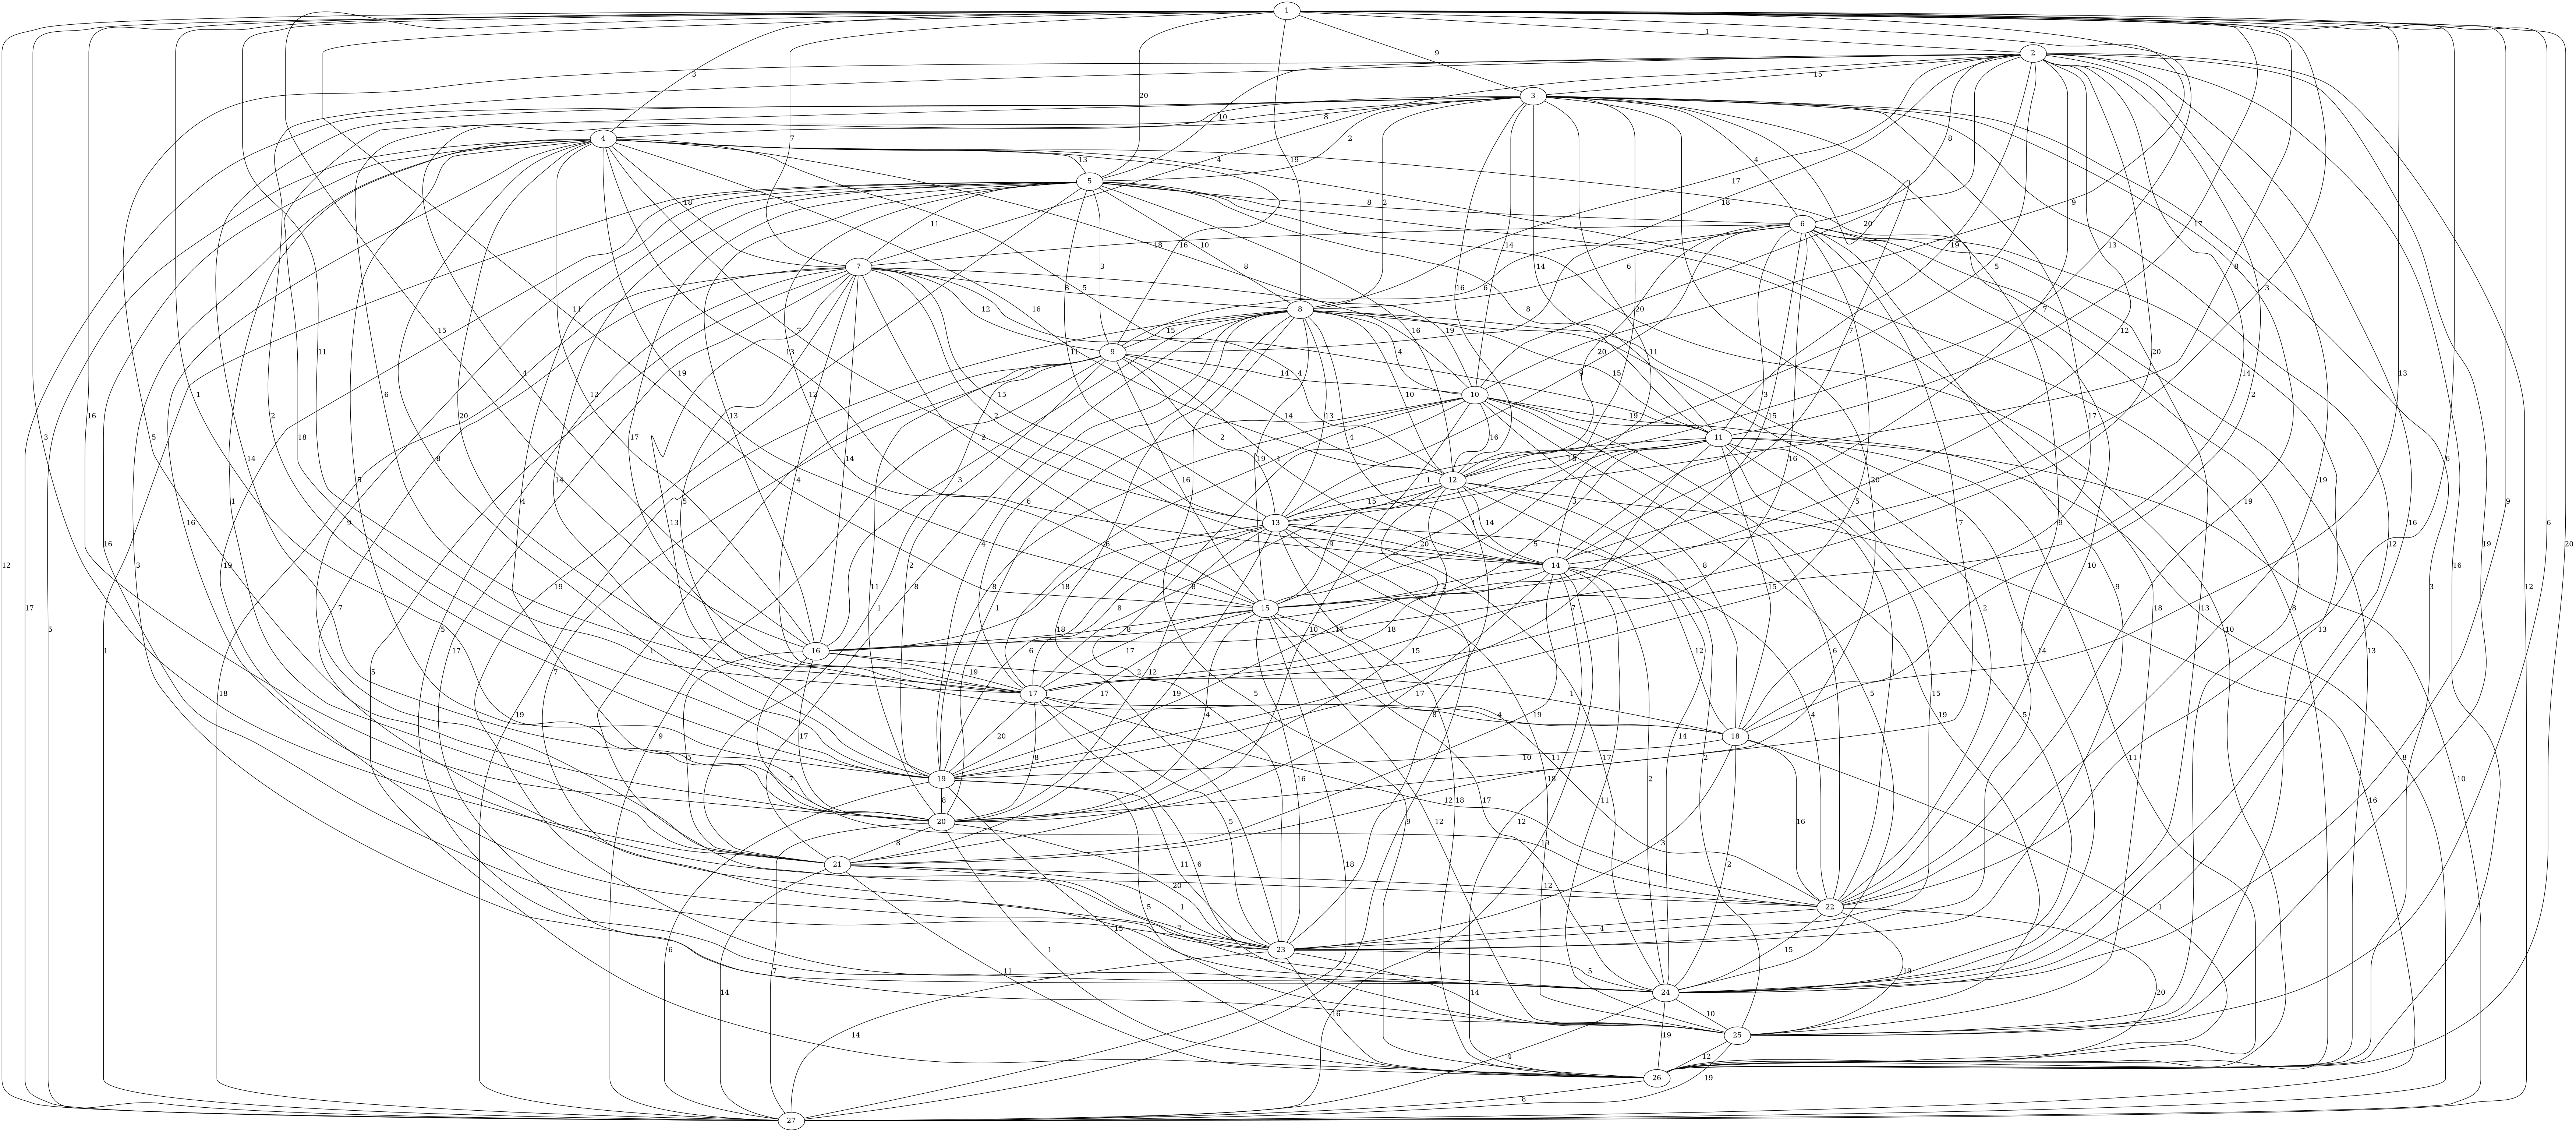
\includegraphics[width=300pt]{graph_size_27_1.png}
		\caption{Граф 1 с 27 вершинами.}
	\end{figure}
	\begin{figure}[h]
		\centering
		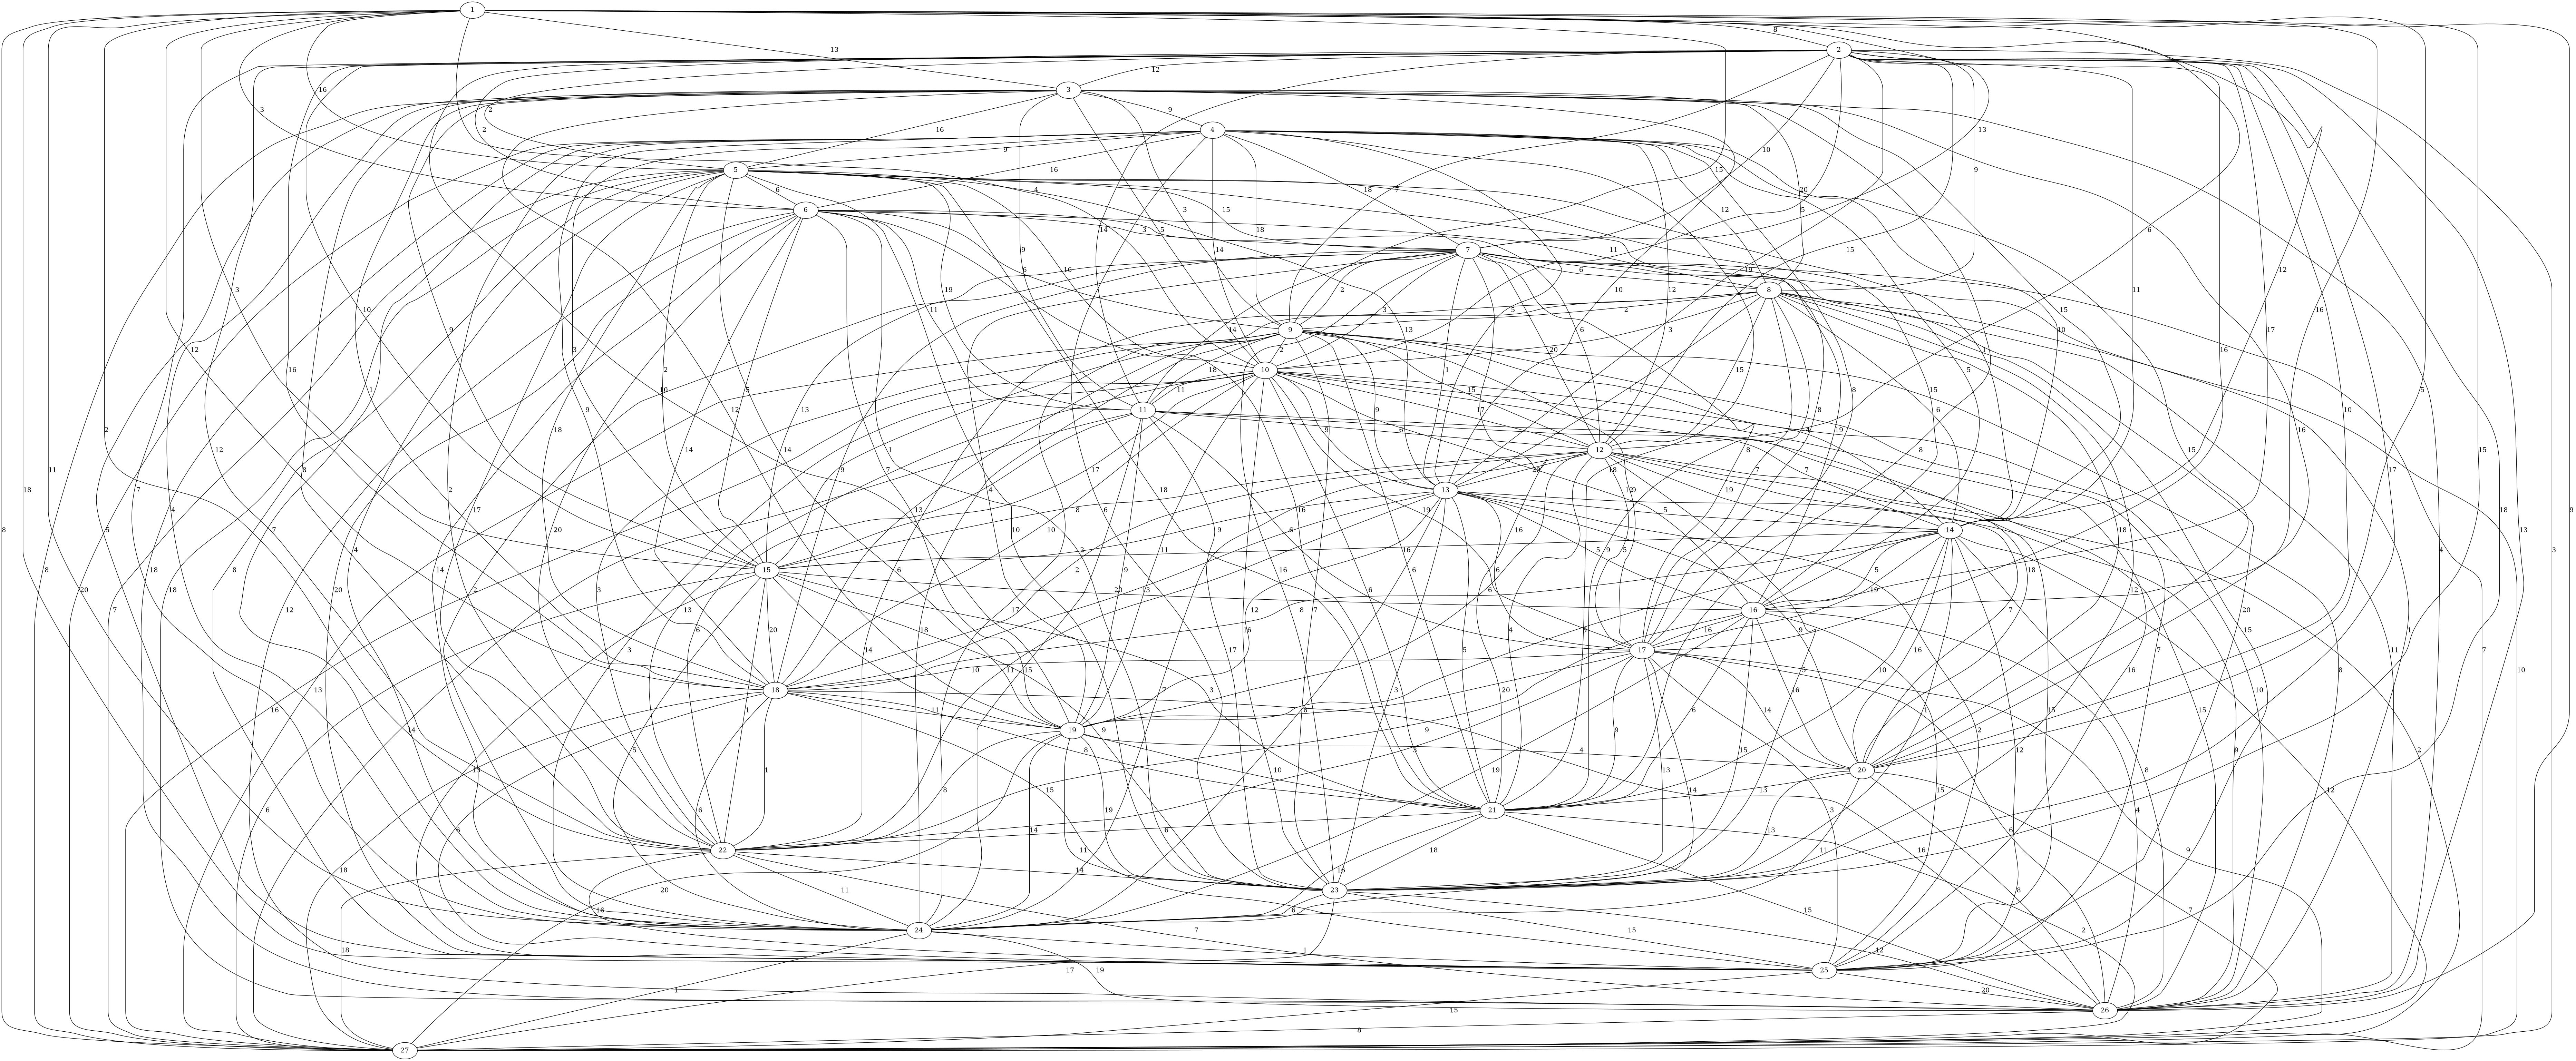
\includegraphics[width=300pt]{graph_size_27_2.png}
		\caption{Граф 2 с 27 вершинами.}
	\end{figure}
	\begin{figure}[h]
		\centering
		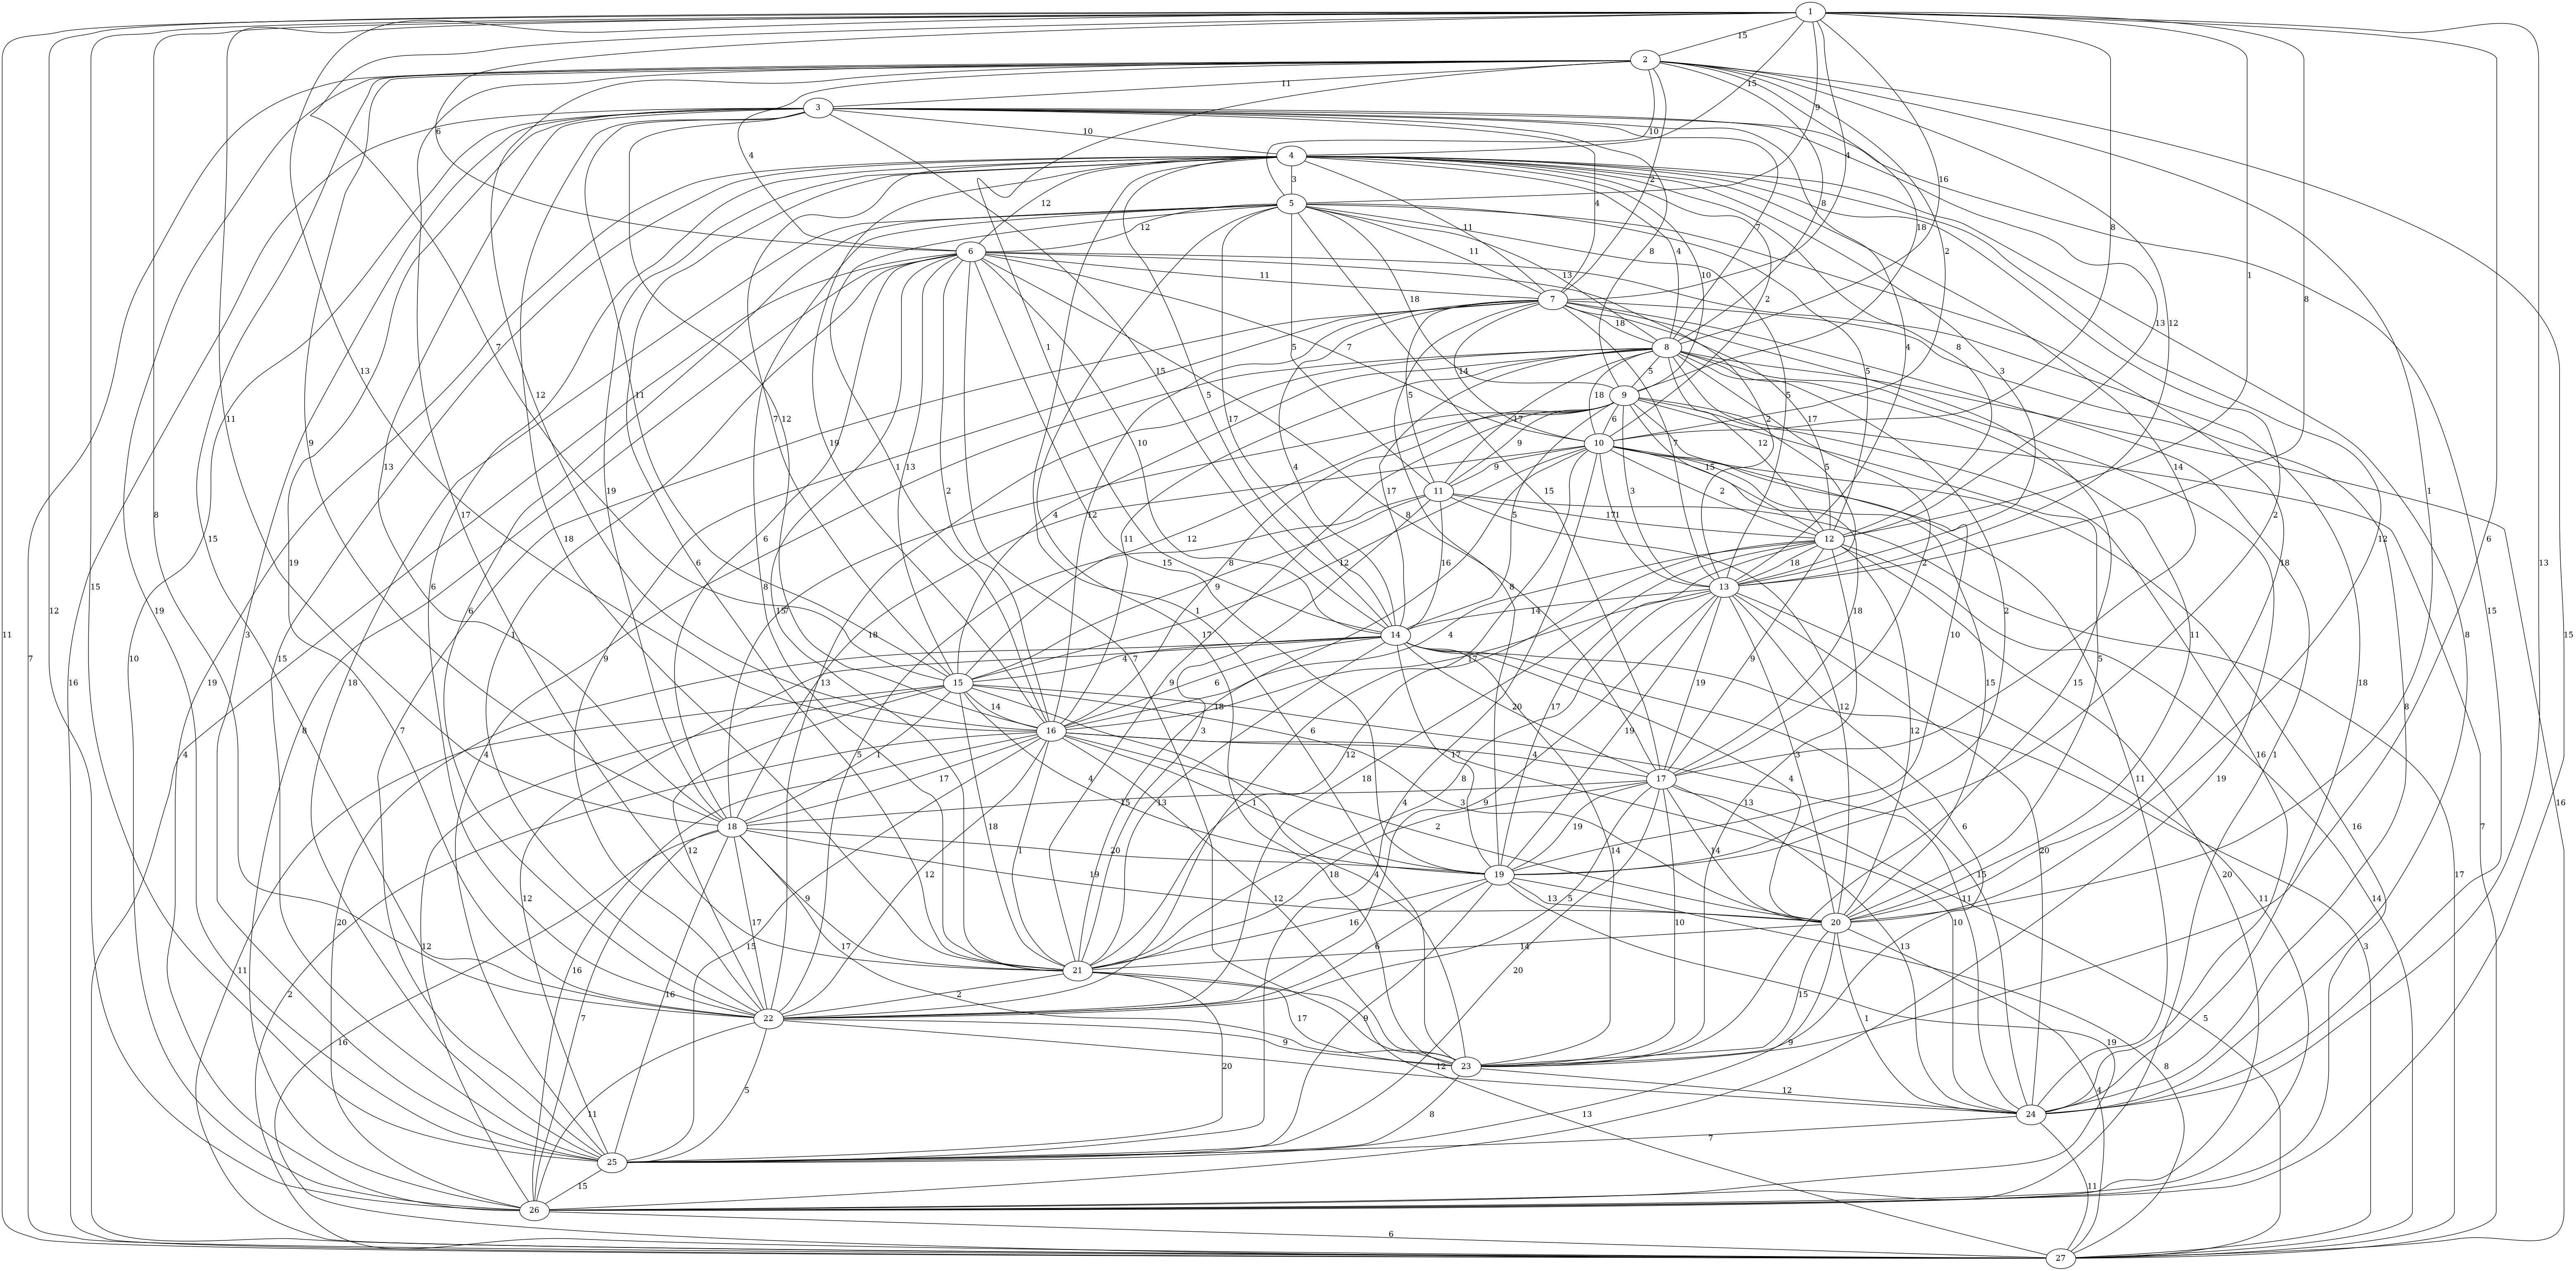
\includegraphics[width=300pt]{graph_size_27_3.png}
		\caption{Граф 3 с 27 вершинами.}
	\end{figure}
	\begin{figure}[h]
		\centering
		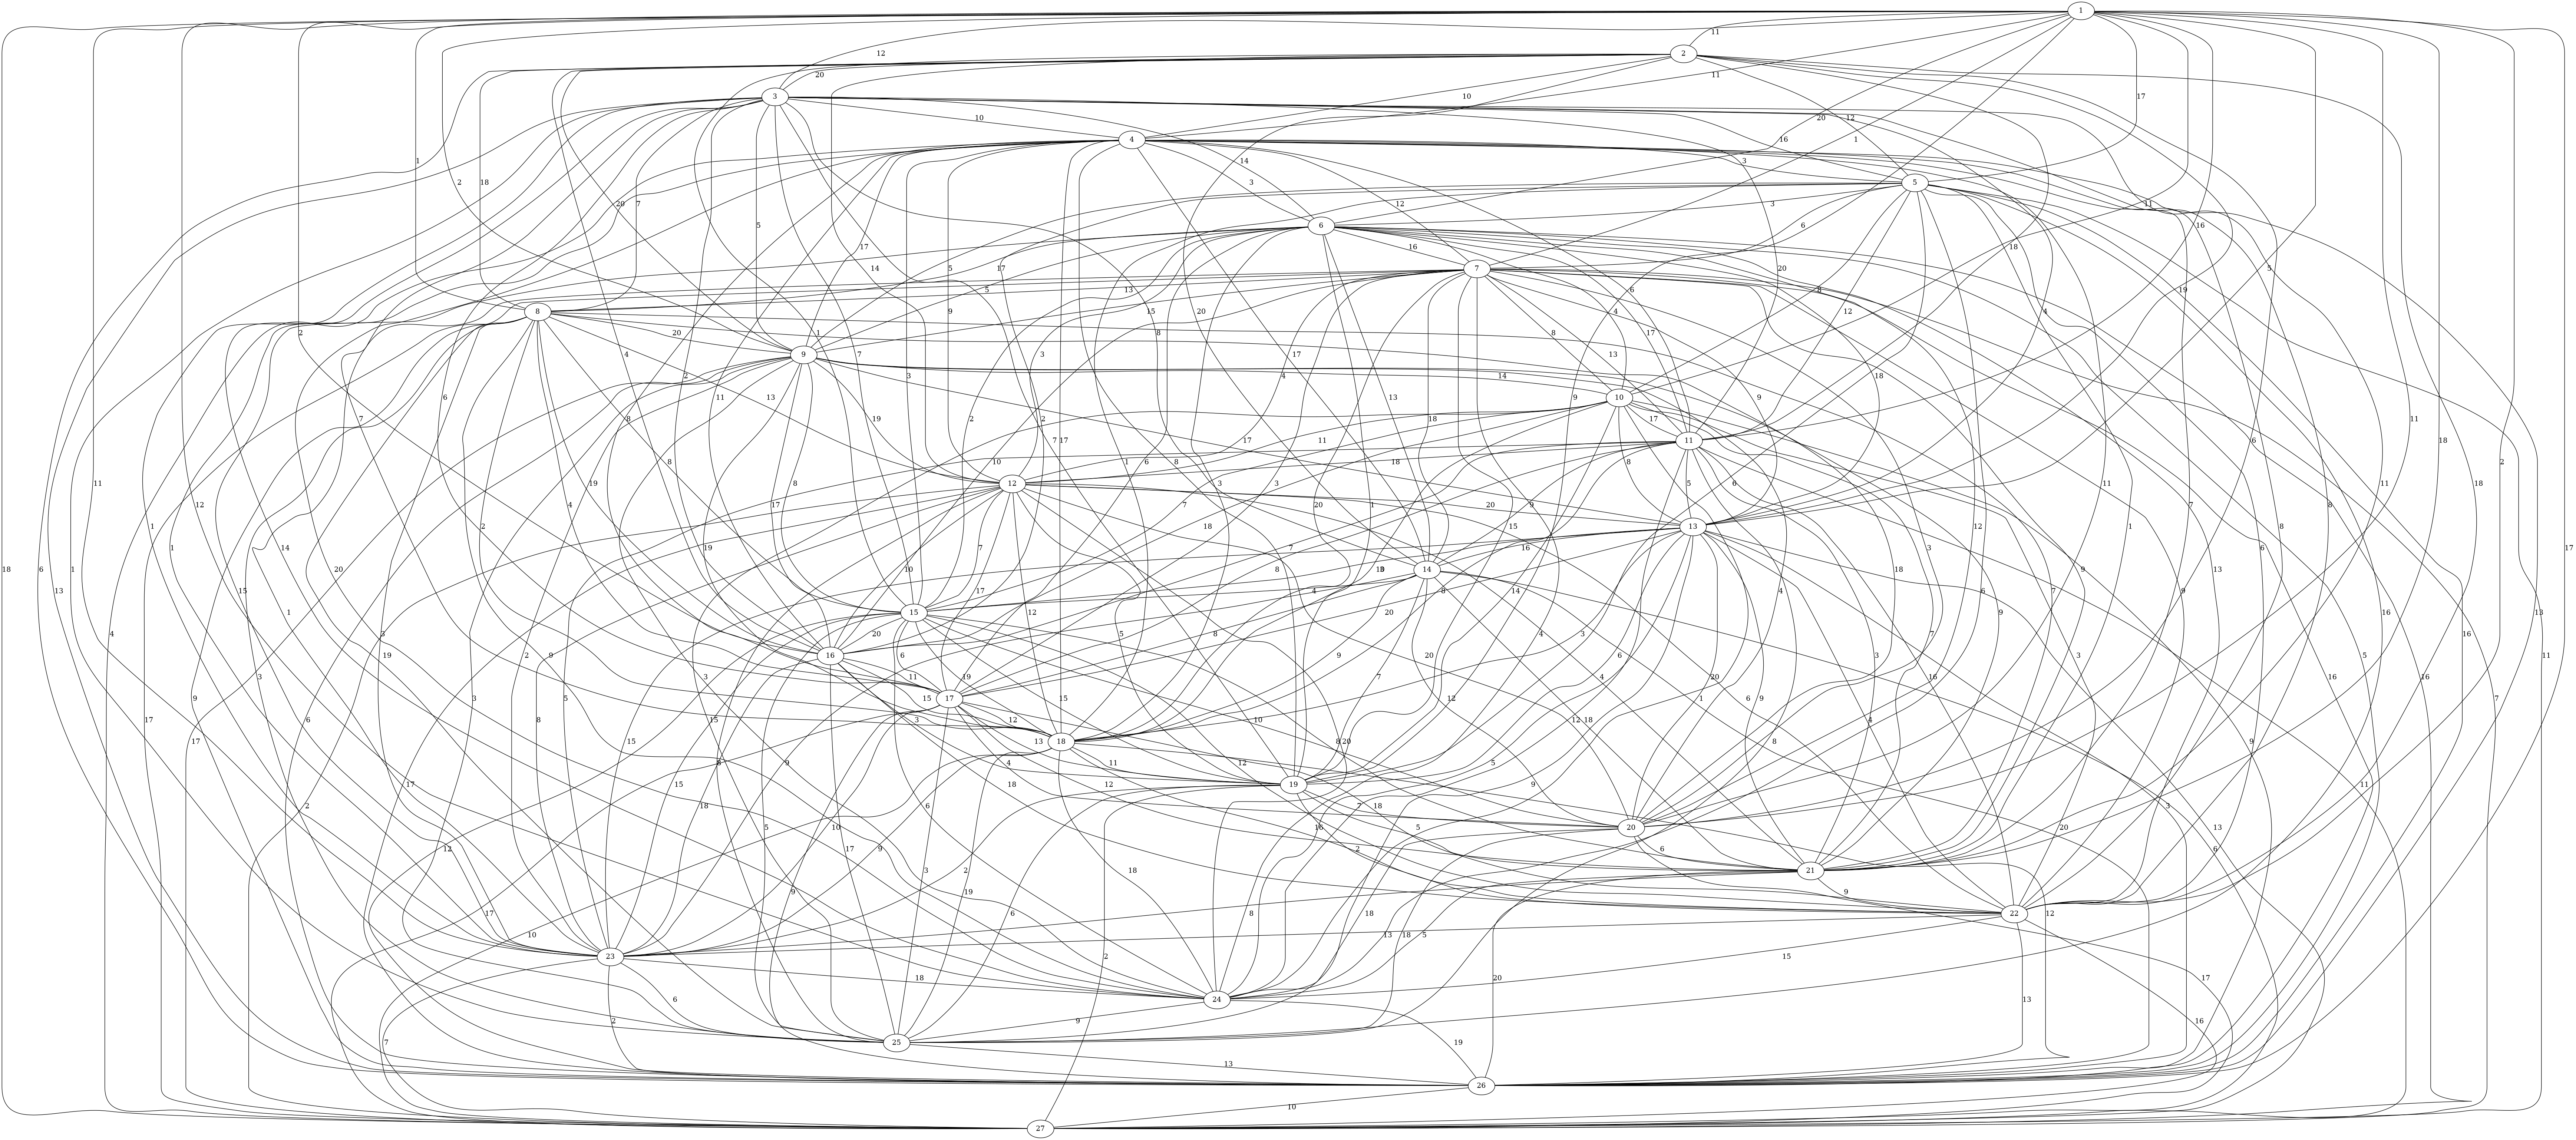
\includegraphics[width=300pt]{graph_size_27_4.png}
		\caption{Граф 4 с 27 вершинами.}
	\end{figure}
	\begin{figure}[h]
		\centering
		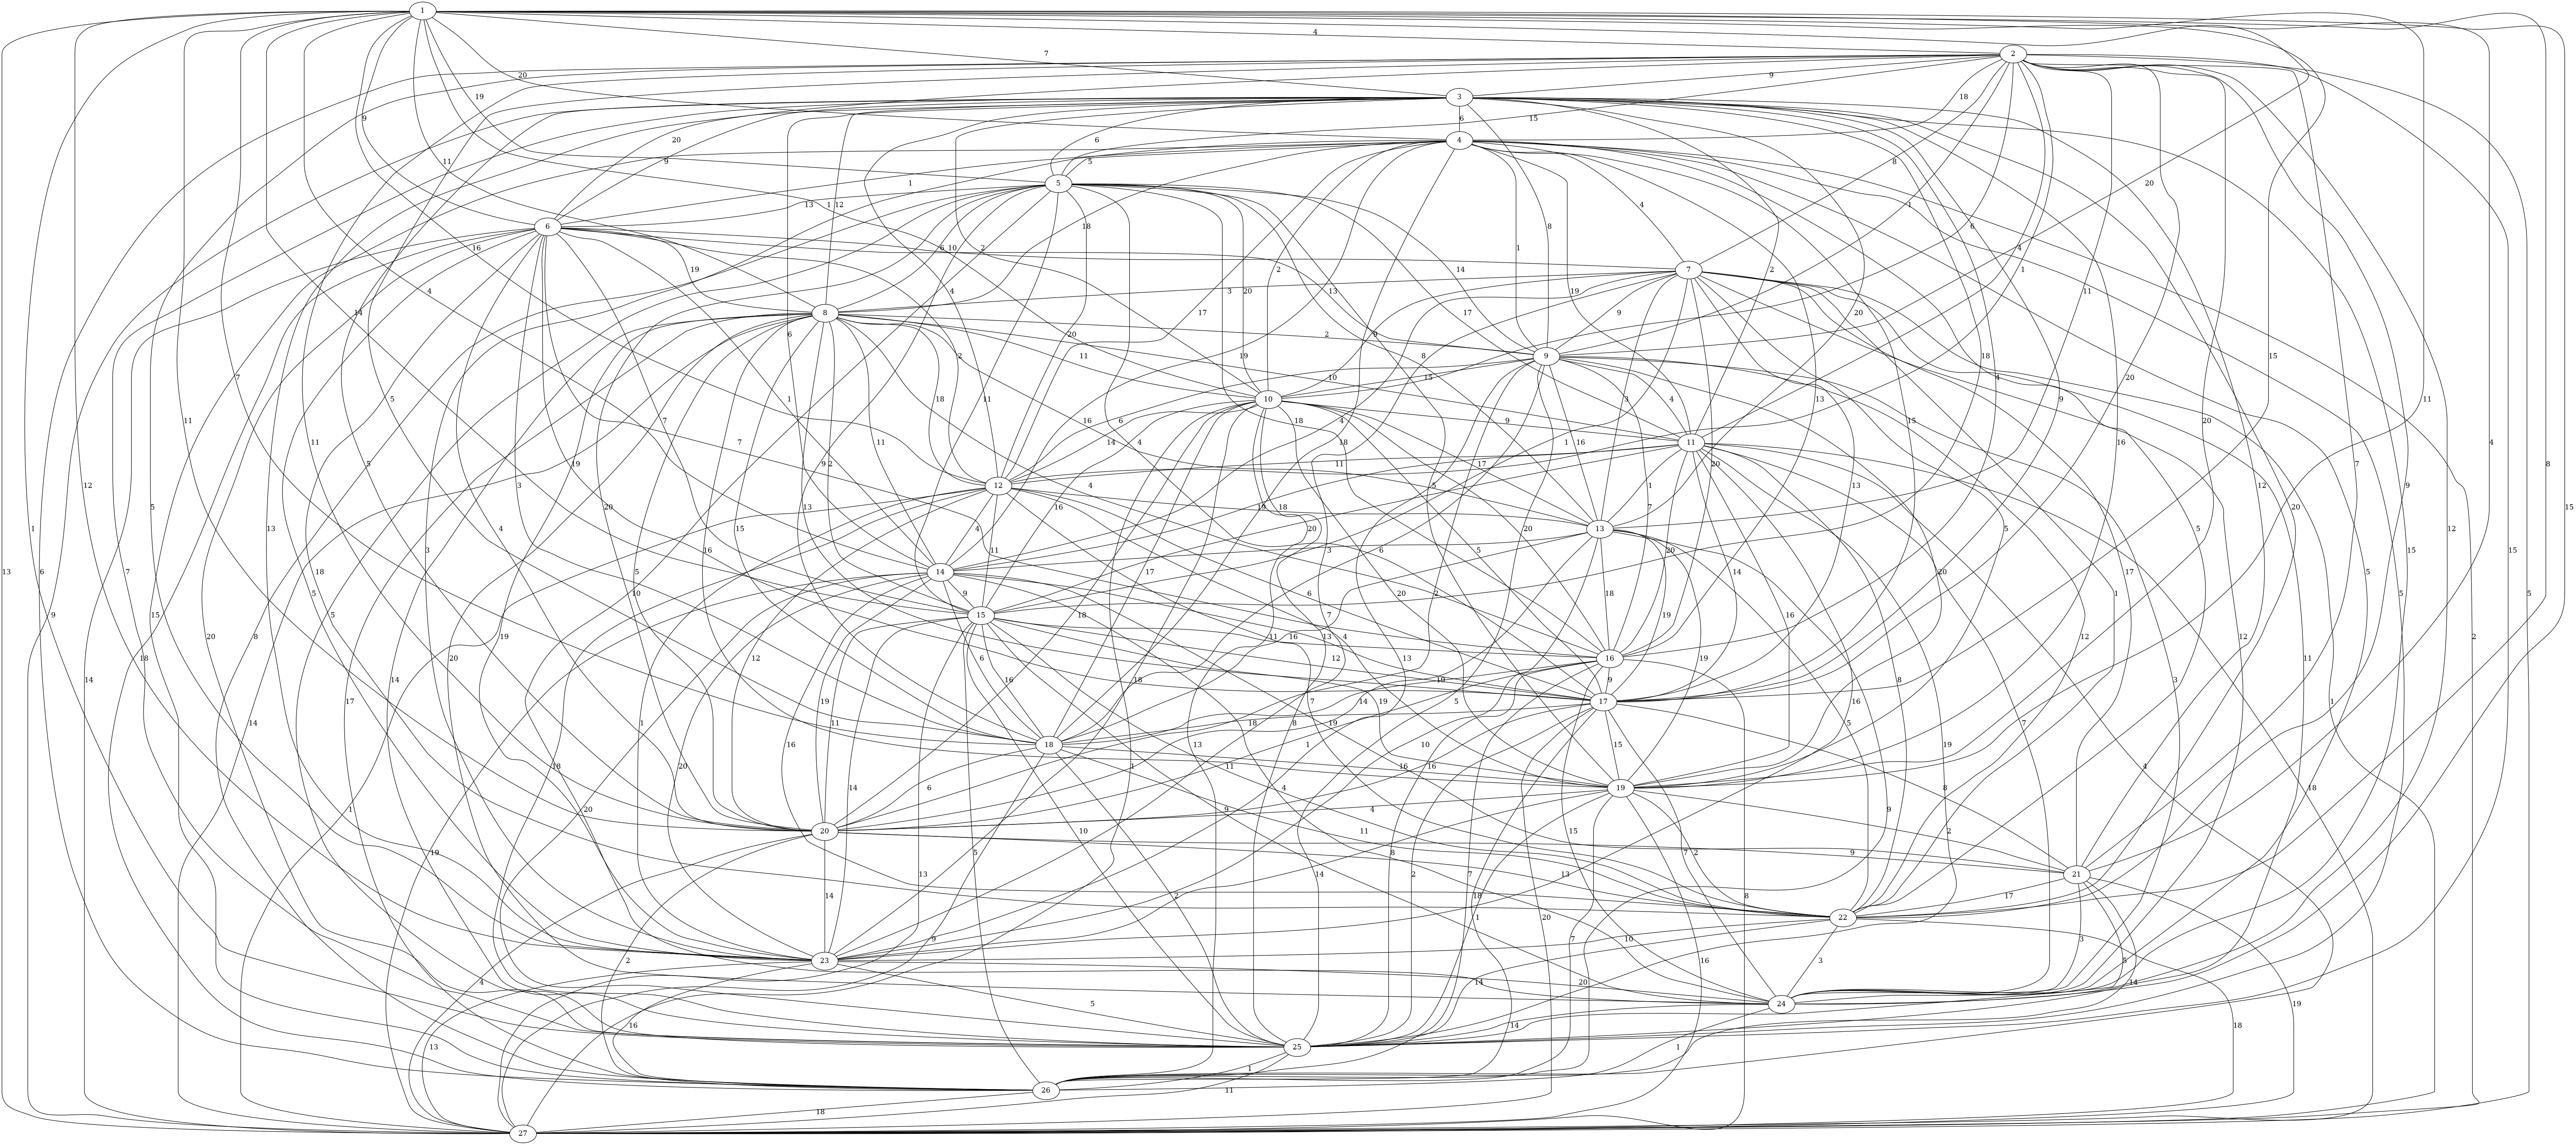
\includegraphics[width=300pt]{graph_size_27_5.png}
		\caption{Граф 5 с 27 вершинами.}
	\end{figure} 

	\vfill
	\clearpage

	\section*{Выводы}
	\addcontentsline{toc}{section}{Выводы}
	В ходе лабораторной работы я познакомился с алгоритмом Флойда-Уоршелла, который предназначен для получения кратчайших путей между всеми парами вершин, существующих в графе. \par
	Из графика оказалось видно, что время выполнения увеличивается согласно ассимптотической сложности алгоритма, т.е. \( N^3 \) с увеличением количества вершин в графе. \par
	Поэтому он довольно эффективен для графов с небольшим количеством вершин.
\end{document}
